The Toric Code is an exactly soluble spin model with $\mathbb{Z}_2$ topological order that was introduced by Alexei Kitaev \cite{cite:fault_tolerant_quantum_computation_by_anyons}. The model is defined on the square lattice with periodic boundary conditions, where on each edge of the lattice there sits a spin-1/2 degree of freedom. Two operators are introduced, the \textit{star operators}
\begin{equation}
	\label{eq:star_operator}
	\hat{A}_+ \coloneqq \sum_{j\in+}\hat{\sigma}_j^z
\end{equation}
and the \textit{plaquette operators}
\begin{equation}
	\label{eq:plaquette_operator}
	\hat{B}_{\scalebox{0.6}{$\square$}} \coloneqq \sum_{j\in \scalebox{0.6}{$\square$}} \hat{\sigma}_j^x,
\end{equation}
where the sums are performed over the four spins connected in a star or plaquette pattern respectively (see Figure \figref{fig:toric_code_star_and_plaquette_operators}) and $\hat{\sigma}_j^x, \hat{\sigma}_j^z$ are Pauli matrices. The Hamiltonian of the Toric Code model is then defined as
\begin{equation}
	\label{eq:toric_code_hamiltonian}
	H_\text{TC} \coloneqq -\sum_+\hat{A}_+ - \sum_{\scalebox{0.6}{$\square$}}\hat{B}_{\scalebox{0.6}{$\square$}},
\end{equation}
where the sums go over all possible stars and plaquettes respectively. 
\begin{figure}
	\centering
	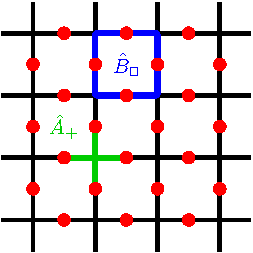
\includegraphics[scale=1]{figures/tikz/toric_code/toric_code_general/toric_code_general.pdf}
	\caption{The Toric Code model is defined on the square lattice with spin-1/2 degrees of freedom living on the edges. the star and plaquette operators \eqref{eq:star_operator} and \eqref{eq:plaquette_operator} act on the four spins arranged in a star or plaquette shape respectively.}
	\label{fig:toric_code_star_and_plaquette_operators}
\end{figure}
Because an arbitrary star and plaquette operator share either two or zero spins, all terms of the Hamiltonian commute and it is thus possible to find the ground state of the model by diagonalizing all terms simultaneously. To diagonalize the star operators $\hat{A}_+$ we choose a basis of $\hat{\sigma}_z$-eigenstates $\ket{i} \in \left\{\ket{\uparrow}, \ket{\downarrow}\right\}$ with eigenvalues $\left\langle\hat{\sigma}_z\right\rangle_i = s_i = \pm 1$ for each spin $i$. In this basis every star operator is diagonal with eigenvalues
\begin{equation}
	\label{eq:toric_code_star_operator_expectation value}
	\langle \hat{A}_+\rangle = \prod_{j\in+}s_j = \pm 1
\end{equation}
To obtain the expectation value $\langle \hat{A}_+\rangle = 1$, the number of spins in the down state $s_j = -1$ around the vertex $+$ must be even. Basis states $\ket{s}$ that give an expectation value of $1$ for every star operator simultaneously are thus the states with an even number of down-spins around every vertex,
\begin{equation}
	\label{eq:toric_code_A_operator_condition}
	\ket{s} = \ket{s_1} \otimes \dots \otimes \ket{s_N}, \quad \prod_{j\in+}s_j = 1 \,\,\,\,\forall +.
\end{equation}
The plaquette operator $\hat{B}_{\scalebox{0.6}{$\square$}}$ acts on such a state $\ket{s}$ state by flipping all spins around the plaquette $\scalebox{0.6}{$\square$}$. Because a plaquette and a star share either zero or two spins, applying an plaquette operator to a state $\ket{s}$ satisfying condition \eqref{eq:toric_code_A_operator_condition} produces a state $\ket{s^\prime}$ that again satisfies \eqref{eq:toric_code_A_operator_condition}, and applying the same plaquette operator a second time produces the initial state $\ket{s}$. If we now take the equal weighted superposition $\ket{\Psi} = \left(\ket{s}+\ket{s^\prime}\right)/\sqrt{2}$, the expectation value of $\hat{B}_{\scalebox{0.6}{$\square$}}$ becomes $\langle \hat{B}_{\scalebox{0.6}{$\square$}}\rangle = 1$.
The ground state of the Hamiltonian \eqref{eq:toric_code_hamiltonian} is thus given by the equal weighted superposition of all basis states satisfying condition \eqref{eq:toric_code_A_operator_condition}. \par
One can show that the ground state can be written as
\begin{equation}
	\ket{\Psi_0} \propto \prod_{\scalebox{0.6}{$\square$}}\left(\id + \hat{B}_{\scalebox{0.6}{$\square$}}\right) \ket{\uparrow} \otimes \dots \otimes \ket{\uparrow}.
\end{equation}
Note that this is also the ground state for the model if open boundary conditions are chosen instead of periodic boundary conditions. \par
For periodic boundary conditions, which is equivalent to putting the model on a torus, one can further show that the ground state is fourfold topologically degenerate. To move from one degenerate section of the Hilbert space to another one must apply a string of operators, wrapping once around the torus. This is a highly non-local operation. Because perturbations are usually local, the toric code model can be interpreted as a form of hardware level error correction. The toric code is considered a topological quantum error correction code and can in theory be used for quantum memory. One can further implement quantum gates acting on the 4-dimensional ground state space by locally creating a pair of anyonic excitations, moving one of the excitations around the torus, and annihilating it with the other one \cite{cite:fault_tolerant_quantum_computation_by_anyons}. Unfortunately, the gates that can be implemented as such do not form a complete gate set and thus do not allow for universal quantum computing. Nevertheless, the Toric code is an important model for the study of topological order and anyonic excitations.